% \documentclass[8pt, aspectratio=169, handout]{beamer} \setbeameroption{show notes on second screen}
% \documentclass[8pt, aspectratio=169, handout]{beamer} \setbeameroption{show only notes}
\documentclass[8pt, aspectratio=169]{beamer}

% MIC Lab template
\input{../template/macros/macros_general.tex}
\input{../template/macros/macros_math.tex}
\input{../template/symbols/symbols_NN.tex}
\input{../template/symbols/symbols_robot.tex}

% Block options: block, alertblock, exampleblock

%~~~~~~~~~~~~~~~~~~~~~~~~~~~~~~~~~~~~~~~~~~~~~~~~~~~~~~~~~~~~~~~~~~~~~~~~~~~~~~
% Use roboto Font (recommended)
% \usepackage[sfdefault]{roboto}
\usepackage[utf8]{inputenc}
\usepackage[T1]{fontenc}
%~~~~~~~~~~~~~~~~~~~~~~~~~~~~~~~~~~~~~~~~~~~~~~~~~~~~~~~~~~~~~~~~~~~~~~~~~~~~~~

%~~~~~~~~~~~~~~~~~~~~~~~~~~~~~~~~~~~~~~~~~~~~~~~~~~~~~~~~~~~~~~~~~~~~~~~~~~~~~~
% Define where theme files are located. ('/styles')
\usepackage{styles/fluxmacros}
\usefolder{styles}
% Use Flux theme v0.1 beta
% Available style: asphalt, blue, red, green, gray, dding (custom)
\usetheme[style=dding]{flux}
%~~~~~~~~~~~~~~~~~~~~~~~~~~~~~~~~~~~~~~~~~~~~~~~~~~~~~~~~~~~~~~~~~~~~~~~~~~~~~~

%~~~~~~~~~~~~~~~~~~~~~~~~~~~~~~~~~~~~~~~~~~~~~~~~~~~~~~~~~~~~~~~~~~~~~~~~~~~~~~
% Extra packages for the demo:
\usepackage{booktabs}
\usepackage{colortbl}
\usepackage{ragged2e}
\usepackage{schemabloc}
\usepackage{multirow}
%~~~~~~~~~~~~~~~~~~~~~~~~~~~~~~~~~~~~~~~~~~~~~~~~~~~~~~~~~~~~~~~~~~~~~~~~~~~~~~

%~~~~~~~~~~~~~~~~~~~~~~~~~~~~~~~~~~~~~~~~~~~~~~~~~~~~~~~~~~~~~~~~~~~~~~~~~~~~~~
% for video
\usepackage{media9}
%~~~~~~~~~~~~~~~~~~~~~~~~~~~~~~~~~~~~~~~~~~~~~~~~~~~~~~~~~~~~~~~~~~~~~~~~~~~~~~

%~~~~~~~~~~~~~~~~~~~~~~~~~~~~~~~~~~~~~~~~~~~~~~~~~~~~~~~~~~~~~~~~~~~~~~~~~~~~~~
% colors
% https://latexcolor.com % color list
\definecolor{airforceblue}{rgb}{0.36, 0.54, 0.66}
\definecolor{awesome}{rgb}{1.0, 0.13, 0.32}
\newcommand{\ctxt}[2]{\color{#1}{#2}\color{black}}
% \newcommand{\mtxt}[2]{\color{#1}\mathbf{#2}\color{black} }
%~~~~~~~~~~~~~~~~~~~~~~~~~~~~~~~~~~~~~~~~~~~~~~~~~~~~~~~~~~~~~~~~~~~~~~~~~~~~~~

%~~~~~~~~~~~~~~~~~~~~~~~~~~~~~~~~~~~~~~~~~~~~~~~~~~~~~~~~~~~~~~~~~~~~~~~~~~~~~~
% Title page details: 
\title{
    Imposing a Weight Norm Constraint for Neuro-Adaptive Control 
} 
\subtitle{
    \textit{IEEE European Control Conference (ECC) 2025}\\
}
\author{
  \textbf{\ctxt{airforceblue}{Myeongseok Ryu}}\inst{1}, Jiyun Kim\inst{2}, and Kyunghwan Choi\inst{1}
  }
\date{2025-06-25}
\institute{%
    \begin{minipage}[c]{\linewidth}
        \centering
        \inst{1}%
        Mobility Intelligence and Control Laboratory (MIC Lab) \\
        % Department of Mechanical and Robotics Engineering\\
        % Gwangju Institute of Science and Technology
        CCS Graduate School of Mobility \\
        Korea Advanced Institute of Science and Technology (KAIST)
        \and
        \inst{2}%
        AI Graduate School\\
        Gwangju Institute of Science and Technology (GIST)
  \end{minipage}
}
%~~~~~~~~~~~~~~~~~~~~~~~~~~~~~~~~~~~~~~~~~~~~~~~~~~~~~~~~~~~~~~~~~~~~~~~~~~~~~~

%~~~~~~~~~~~~~~~~~~~~~~~~~~~~~~~~~~~~~~~~~~~~~~~~~~~~~~~~~~~~~~~~~~~~~~~~~~~~~~
% Global settings

% \titlegraphic{assets/MIC_Lab_logo.png}
\titlegraphic{assets/MIC_Lab_logo_white.png}

% make institute font size smaller
\setbeamerfont{institute}{size=\normalsize}

\AtBeginSection[]{%
  \frame<beamer>{ 
    \frametitle{Outline}   
    \tableofcontents[currentsection] 
  }
}

% \AtBeginSubsection[]{%
%   \begin{frame}
%   \vfill
%   \centering
%     \insertsectionhead
%     \\
%     \large\textbf{\insertsubsectionhead}
%   \vfill
%   \end{frame}
% }
%~~~~~~~~~~~~~~~~~~~~~~~~~~~~~~~~~~~~~~~~~~~~~~~~~~~~~~~~~~~~~~~~~~~~~~~~~~~~~~

\begin{document}

%~~~~~~~~~~~~~~~~~~~~~~~~~~~~~~~~~~~~~~~~~~~~~~~~~~~~~~~~~~~~~~~~~~~~~~~~~~~~~~
% Title page frame
\titlepage 

% Outline frame
\begin{frame}{Outline}
  \tableofcontents
\end{frame}
%~~~~~~~~~~~~~~~~~~~~~~~~~~~~~~~~~~~~~~~~~~~~~~~~~~~~~~~~~~~~~~~~~~~~~~~~~~~~~~

% ╔═══════════════════════════════════════════════╗
% ║ Section: Background and Contributions         ║
% ╚═══════════════════════════════════════════════╝

\section{Background and Contributions}

\subsection{Introduction to Neuro-Adaptive Control}

%~~~~~~~~~~~~~~~~~~~~~~~~~~~~~~~~~~~~~~~~~~~~~~~~~~~~~~~~~~~~~~~~~~~~~~~~~~~~~~
\begin{frame}{\insertsubsectionhead}{What is Neuro-Adaptive Control?}

  \textbf{Neuro-Adaptive Control}
  \small{
    \begin{itemize}
      \item \textbf{Neuro-adaptive control} (NAC) is a control strategy that combines \ctxt{airforceblue}{neural networks (NNs) } with \ctxt{awesome}{adaptive control } \cite{Farrell:2006aa}.
      \item Features of both \ctxt{airforceblue}{NNs } and \ctxt{awesome}{adaptive control } can be found in NAC.
    \end{itemize}
  }

  \begin{figure}
    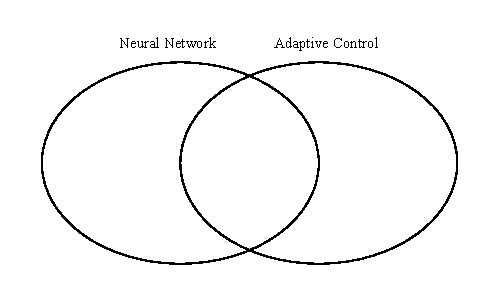
\includegraphics[width=0.65\textwidth]{figures/NAC.drawio.pdf}
  \end{figure}
  
\end{frame} 
%~~~~~~~~~~~~~~~~~~~~~~~~~~~~~~~~~~~~~~~~~~~~~~~~~~~~~~~~~~~~~~~~~~~~~~~~~~~~~~

\note[enumerate]
{
  \item adaptive controls adapts their parameters in real-time to systems.
  \begin{itemize}
    \item Hence, they can handle uncertainties and disturbances.
  \end{itemize}
  \item Like adaptive control, NAC adapts its NN weights, as well.
  \item Hence, it has both features of NN and adaptive control.
}

%~~~~~~~~~~~~~~~~~~~~~~~~~~~~~~~~~~~~~~~~~~~~~~~~~~~~~~~~~~~~~~~~~~~~~~~~~~~~~~
\begin{frame}{\insertsubsectionhead}{What is Neuro-Adaptive Control?}

  \textbf{Advantages of Neuro-Adaptive Control}
  \small{
    \begin{itemize}
      \item <2-> \textbf{Adaptability}: NAC adapts \ctxt{airforceblue}{NN weights }to changing environments and system dynamics.
      \item <3-> \textbf{Stability Guarantee}: The closed-loop stability is ensured using \ctxt{airforceblue}{Lyapunov stability theory}.
      \item <4-> \textbf{Online Learning Capability}: NAC adapts in \ctxt{airforceblue}{real-time } to new data with stability guarantees.
      \item <5-> \textbf{Robustness}: NAC handles \ctxt{airforceblue}{uncertainties and disturbances }effectively with adaptive control techniques.
    \end{itemize}
  }
  
\begin{figure}
  \label{fig:general_framework}
  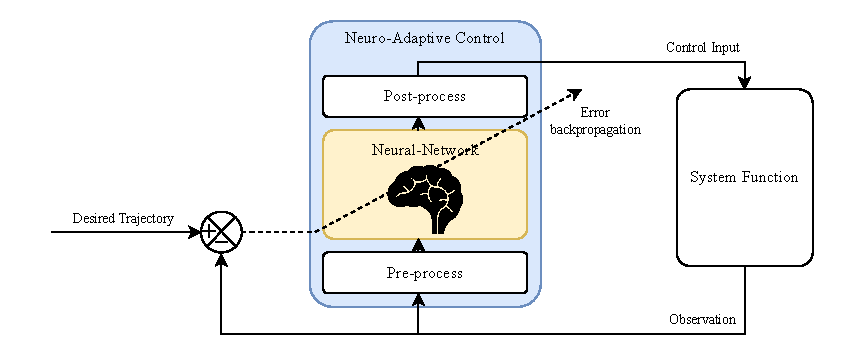
\includegraphics[width=0.65\textwidth]{figures/conv_nac.drawio.pdf}
  \caption{General framework of neuro-adaptive control (NAC).}
\end{figure}

\end{frame}
%~~~~~~~~~~~~~~~~~~~~~~~~~~~~~~~~~~~~~~~~~~~~~~~~~~~~~~~~~~~~~~~~~~~~~~~~~~~~~~

\note[enumerate]
{
  \item The features are...
  \begin{itemize}
    \item It can adapts its weights to change environments.
    \item And the stability is ensured in the sense of Lyapunov.
    \item So, it has online learning capability.
    \item In addition, with various methods from adaptive control, NAC can be more robust than naive NN-based control methods.
  \end{itemize}
}

%~~~~~~~~~~~~~~~~~~~~~~~~~~~~~~~~~~~~~~~~~~~~~~~~~~~~~~~~~~~~~~~~~~~~~~~~~~~~~~
\begin{frame}{\insertsubsectionhead}{What is Neuro-Adaptive Control?}

  \textbf{Existing Challenges in NAC}

  \begin{enumerate}
    
    \onslide<2->
    {
      \begin{columns}[T,onlytextwidth]

        \column{0.49\textwidth}

          \small{
            \item \textbf{Weight Boundedness:} 

            \begin{itemize}
              \item Generally, NN weights are adapted by \ctxt{airforceblue}{gradient descent method}.
              \begin{itemize}
                \item Objective function typically consists of the control error.
              \end{itemize}
              \item Hence, the NN weights can grow \ctxt{awesome}{unbounded}, leading to instability (also known as \textit{parameter drift}).
              \item Unbounded weights can cause the NN to produce \ctxt{airforceblue}{large control inputs}, which may lead to following challenges.
            \end{itemize}
          }
            
          \column{0.49\textwidth}
            \centering

              \begin{figure}
                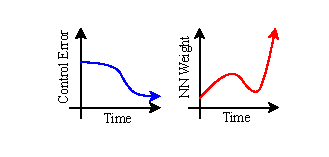
\includegraphics[width=0.7\textwidth]{figures/unbounded.drawio.pdf}
                \caption{Divergence of NN weights even with convergent control error.}
              \end{figure}
        \end{columns}
      }

      \onslide<3->
      {
        \begin{columns}[T,onlytextwidth]
          \column{0.49\textwidth}

          \small{
            \item \textbf{Control Saturation} \textit{(unpredictable amplitude of NN outputs)}: 

            \begin{itemize}
              \item Typical issue of control problem in physical systems.
              \item The NN outputs are \ctxt{awesome}{unpredictable } and \ctxt{awesome}{not interpretable}.
              \item These features—unbounded NN weights and unpredictable amplitudes—can lead to \ctxt{airforceblue}{input saturation}.
            \end{itemize}
          }

          \column{0.49\textwidth}
            \centering
            \begin{figure}
              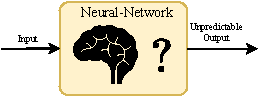
\includegraphics[width=0.8\textwidth]{figures/unpredictable.drawio.pdf}
              \caption{Unpredictable amplitude of NN outputs.}
            \end{figure}
        \end{columns}
      }

  \end{enumerate}

\end{frame}
%~~~~~~~~~~~~~~~~~~~~~~~~~~~~~~~~~~~~~~~~~~~~~~~~~~~~~~~~~~~~~~~~~~~~~~~~~~~~~~

\note[enumerate]
{
  \item However, there are some challenges in NAC.
  \item The first challenge is weight boundedness.
  \begin{itemize}
    \item If the NNs are used for control naively, the boundedness of NN weights is not ensured.
    \item For instance, despite the convergence of the control error, the NN weights can diverge like parameter drift.
    \item This divergence leads to the following issue.
  \end{itemize}
  \item Second one is the NN's output can be excessively large control inputs.
  \begin{itemize}
    \item This is because, the output of NN is not interpretable and unpredictable.
    \item So, the input saturation problem can occur by them.
  \end{itemize}
}

% ╔═══════════════════════════════════════════════╗
% ║ Section: Background and Contributions         ║
% ║   - Subsection: Literature Review             ║
% ╚═══════════════════════════════════════════════╝
\subsection{Literature Review}

%~~~~~~~~~~~~~~~~~~~~~~~~~~~~~~~~~~~~~~~~~~~~~~~~~~~~~~~~~~~~~~~~~~~~~~~~~~~~~~
\begin{frame}{\insertsubsectionhead}
  
  \begin{enumerate}

    \begin{columns}[T]

        \column{0.33\textwidth}
          \item \textbf{Projection Operator} \small{\textit{for weight boundednss}}

          \onslide<2->
          {
            \begin{itemize}
              \item Projects the NN weights onto a convex set.
              \item Ensures that the weights \ctxt{airforceblue}{remain }within a predefined bound.
            \end{itemize}

            \begin{equation}
              \estwth \leftarrow \myproj_{\overline{\theta}}(\estwth)
            \end{equation}
          }

        \column{0.33\textwidth}
          \item \textbf{$\sigma$-modification, and $\epsilon$-modification} \small{\textit{for weight boundednss}}

          \onslide<3->
          {
            \begin{itemize}
              \item Add a \ctxt{airforceblue}{stabilizing term }(\eg $ -\lambda \estwth $) to adaptation law.
              \item Construct a \ctxt{airforceblue}{invariant set }of the NN weights.
            \end{itemize}

            \begin{equation}
              \ddtt{\estwth} \leftarrow \ddtt{\estwth} - \ctxt{awesome}{\lambda \estwth}
            \end{equation}
          }

        \column{0.33\textwidth}
          \item \textbf{Additional Control Inputs} \small{\textit{for control saturation}}

          \onslide<4->
          {
            \begin{itemize}
              \item \ctxt{airforceblue}{Conventional controllers }are used to address control input saturation. 
                    \begin{itemize}
                      \item Barrier Lyapunov function or auxiliary system-based control inputs.
                    \end{itemize}
              \item In general, \ctxt{awesome}{nominal models }are required.
            \end{itemize}
          }

      \end{columns}

  \end{enumerate}

  % \vspace{0.5cm}

  \begin{columns}[T]

      \column{0.33\textwidth}

        \onslide<2->
        {
          \centering
          \begin{figure}
            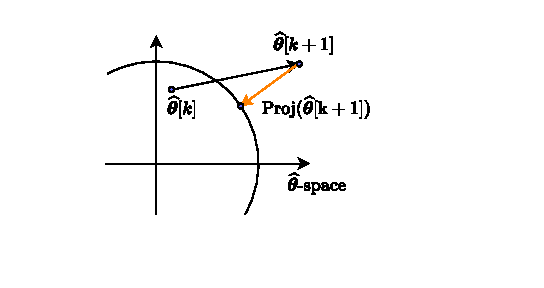
\includegraphics[width=0.8\textwidth]{figures/existing_proj.drawio.pdf}
            \caption{Projection of NN weights on a convex set.}
          \end{figure}
        }

      \column{0.33\textwidth}
          
        \onslide<3->
        {
          \centering
          \begin{figure}
            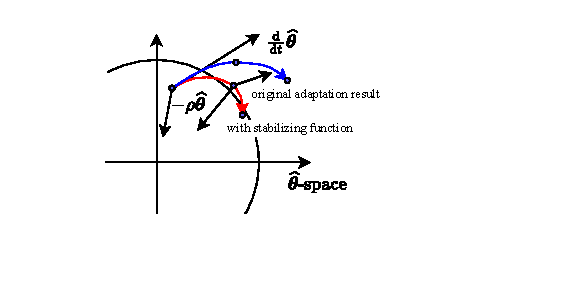
\includegraphics[width=0.8\textwidth]{figures/existing_modi.drawio.pdf}
            \caption{Adaptation result with stabilizing function (\eg $\sigma$-modification).}
          \end{figure}
        }
      
      \column{0.33\textwidth}
      
        \onslide<4->
        {
          \centering
          \begin{figure}
            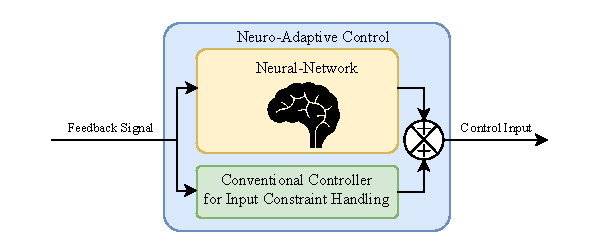
\includegraphics[width=0.999\textwidth]{figures/existing_conv.drawio.pdf}
            \caption{Control input saturation handling with additional control inputs.}
          \end{figure}
        }

    \end{columns}

\end{frame}
%~~~~~~~~~~~~~~~~~~~~~~~~~~~~~~~~~~~~~~~~~~~~~~~~~~~~~~~~~~~~~~~~~~~~~~~~~~~~~~

\note[enumerate]
{
  \item To address these issues, several methods have been introduced.
  \item For weight boundedness, the projection operator and modification methods are used.
  \begin{itemize}
    \item they ensures the weight boundedness by projects onto a convex set or adding a stabilizing term.
    \item Hence, the the boundedness of NN weights can be easily ensured.
  \end{itemize}
  \item For control input saturation, additional control inputs are used.
  \begin{itemize}
    \item Conventionally, auxiliary system-based control inputs or, more recently, barrier Lyapunov function-based control inputs are used.
    \item For this, the nominal model knowledge is required.
    \item These makes the control design more complicated, but, have shown the effectiveness of the control input saturation handling.
  \end{itemize}
}

%~~~~~~~~~~~~~~~~~~~~~~~~~~~~~~~~~~~~~~~~~~~~~~~~~~~~~~~~~~~~~~~~~~~~~~~~~~~~~~
\begin{frame}{\insertsubsectionhead}{Limitations of Existing Methods}

  \onslide<1->
  {
    \textbf{Limitation 1: Lack of Optimality}
  }
  \begin{itemize}
    \item<2-> The existing methods do not guarantee the \ctxt{airforceblue}{optimality } of the control input.
    \item<3-> Projection operator:
    \begin{itemize}
      \item The projection operator \ctxt{awesome}{simply projects } the NN weights onto a convex set, regardless of the imposed \ctxt{airforceblue}{constraints } (\eg weight boundedness or input saturation).
      \item Moreover, if the convex set is conservatively defined, the weights may be limited to a \ctxt{awesome}{suboptimal region}.
    \end{itemize}
    \item<4-> $\sigma$- and $\epsilon$-modification:
    \begin{itemize}
      \item The stabilizing term \ctxt{awesome}{biases } the NN weights towards the origin.
      \item Therefore, the weights converge toward a \ctxt{awesome}{suboptimal point}.
    \end{itemize}
  \end{itemize}

  \onslide<1->
  {
    \textbf{Limitation 2: Disruption of Learning Process by Additional Control Inputs}
  }
  \begin{itemize}
    \item<5-> Feedback tracking error for learning is \ctxt{awesome}{disrupted } by additional control inputs.
      \begin{itemize}
        \item The feedback error \ctxt{airforceblue}{does not reflect } the error induced by the NN, directly.
        \item The additional control inputs may exceeds the \ctxt{awesome}{input saturation limits }, already.
    \end{itemize}  
  \end{itemize}

\end{frame}
%~~~~~~~~~~~~~~~~~~~~~~~~~~~~~~~~~~~~~~~~~~~~~~~~~~~~~~~~~~~~~~~~~~~~~~~~~~~~~~

\note[enumerate]
{
  \item the limitations of the existing methods can be summarized as follows.
  \item Most of methods does not consider the optimality when the constraints are active.
  \begin{itemize}
    \item Because, they only consider the boundedness of the weights or the control input saturation using additional operators or terms.
  \end{itemize}
  \item Using additional terms can lead to disruption of learning process.
  \item It is, because, as the NN learns with respect to the feedback error, once the additional control inputs are applied, the feedback error does not reflect the error induced by the NN, directly.
  \item Moreover, the additional control inputs may exceed the input limits, already.
  \item Therefore, in the worst case, the NN may be forced to compensate for the additional terms.
}

% ╔═══════════════════════════════════════════════╗
% ║ Section: Background and Contributions         ║
% ║   - Subsection: Contributions                 ║
% ╚═══════════════════════════════════════════════╝
\subsection{Contributions}

%~~~~~~~~~~~~~~~~~~~~~~~~~~~~~~~~~~~~~~~~~~~~~~~~~~~~~~~~~~~~~~~~~~~~~~~~~~~~~~
\begin{frame}{\insertsubsectionhead}

  \textbf{Contribution 1: Unified Optimization Framework} 
  \onslide<2->
  {
    \begin{itemize}
      \item Trajectory tracking and constraint handling are formulated as a \ctxt{airforceblue}{unified constrained optimization } problem.
      \item The \ctxt{awesome}{conventional controllers } does not required.
      \begin{itemize}
        \item Nominal model knowledge is not required for the conventional controllers.
      \end{itemize}
    \end{itemize}
  }

  \textbf{Contribution 2: Online Learning Capability (Stability Guarantees)}
  \onslide<3->
  {
    \begin{itemize}
      \item Stability are rigorously proven using \ctxt{airforceblue}{Lyapunov stability theory}.
      \item Hence, \ctxt{airforceblue}{online learning} with \ctxt{awesome}{no prior system knowledge } is possible.
    \end{itemize}
  }

  \textbf{Contribution 3: Weight and Control Input Constraint Handling}
  \onslide<4->
  {
    \begin{itemize}
      \item Weight and control input \ctxt{awesome}{constraints } are \ctxt{airforceblue}{explicitly considered } in the optimization problem.
      \item \ctxt{airforceblue}{Any combination } of convex input constraints can be handled.
    \end{itemize}
  }

\end{frame}
%~~~~~~~~~~~~~~~~~~~~~~~~~~~~~~~~~~~~~~~~~~~~~~~~~~~~~~~~~~~~~~~~~~~~~~~~~~~~~~

\note[enumerate]
{
  \item So, here are the contributions of this work.
  \item We, first, formulated a unified optimization framework for trajectory tracking and constraint handling.
  \item Hence, we do not need the additional operators or conventional controllers, which may need the nominal model knowledge.
  \item Second, we rigorously proved the stability of the proposed method using Lyapunov stability theory.
  \item It means, that the proposed method can learn online without any prior system knowledge with stability guarantees.
  \item Finally, as we explicitly consider the weight and control input constraints in the optimization problem, we can handle any combination of convex input constraints and weight constraint.
}

% ╔═══════════════════════════════════════════════╗
% ║ Section: Proposed Method                      ║
% ╚═══════════════════════════════════════════════╝

\section{Proposed Method}

% ╔═══════════════════════════════════════════════╗
% ║ Section: Proposed Method                      ║
% ║   - Subsection: Architecture of the Proposed Method
% ╚═══════════════════════════════════════════════╝
\subsection{Architecture of the Proposed Method}

%~~~~~~~~~~~~~~~~~~~~~~~~~~~~~~~~~~~~~~~~~~~~~~~~~~~~~~~~~~~~~~~~~~~~~~~~~~~~~~
\begin{frame}{\insertsubsectionhead}
  
  \begin{columns}
    
    \column{0.5\textwidth}
      
    \onslide<2->
    {
      \textbf{Target Two-link Robotic Manipulator System}:
      \small{
        \begin{itemize}
          \item Control input \ctxt{awesome}{saturation function } $\mysat(\cdot)$.
          \item Desired trajectory $\mv{q}_d$ is given.
        \end{itemize}
          \begin{equation}\label{eq:sys}
            \mm{M}\ddq + \mm{V}_m\dq + \mv{F} + \mv{G} + \mv{\tau}_d
            =
            \mysat(\mv{\tau})
          \end{equation}    
      }
    }
    
    \onslide<3->
    {
      \textbf{Control Input}:
      \small{
        \begin{itemize}
          \item NN's \ctxt{airforceblue}{output } $\mv{\Phi}$ is used as the control input.
          \item Consists of the \ctxt{awesome}{estimated NN weights } $\estwth$.
        \end{itemize}
        \begin{equation}\label{eq:input}
          \mv{\tau} := \mv{\Phi}(\mv{q}_n; \estwth)
        \end{equation}
      }
    }

    \onslide<4->
    {
      \textbf{Deep Neural Network (DNN)}:
      \small{
        \begin{itemize}
          \item $k$ layers with weights $\estwth_i:=\myvec(\estwV_i)$.
          \item Activation function: $\phi(\cdot):=tanh(\cdot)$.
          \begin{equation}\label{eq:NN}
            \mv{\Phi}(\mv{q}_n; \estwth)
            :=
            \begin{cases}
                \estwV_i^\top \act_i(\estNN_{i-1}), 
                &
                i\in\{1,\dots ,k\},
                \\
                \estwV_0^\top {\q}_n,
                &
                i=0
                ,
            \end{cases}
          \end{equation}
        \end{itemize}
      }
    }

    \column{0.5\textwidth}  

      \begin{figure}
        \includegraphics[width=0.8\textwidth]{figures/Controller.drawio.pdf}
        \caption{Architecture of the proposed method.}
      \end{figure}

    \onslide<4->
    {
      \begin{figure}
        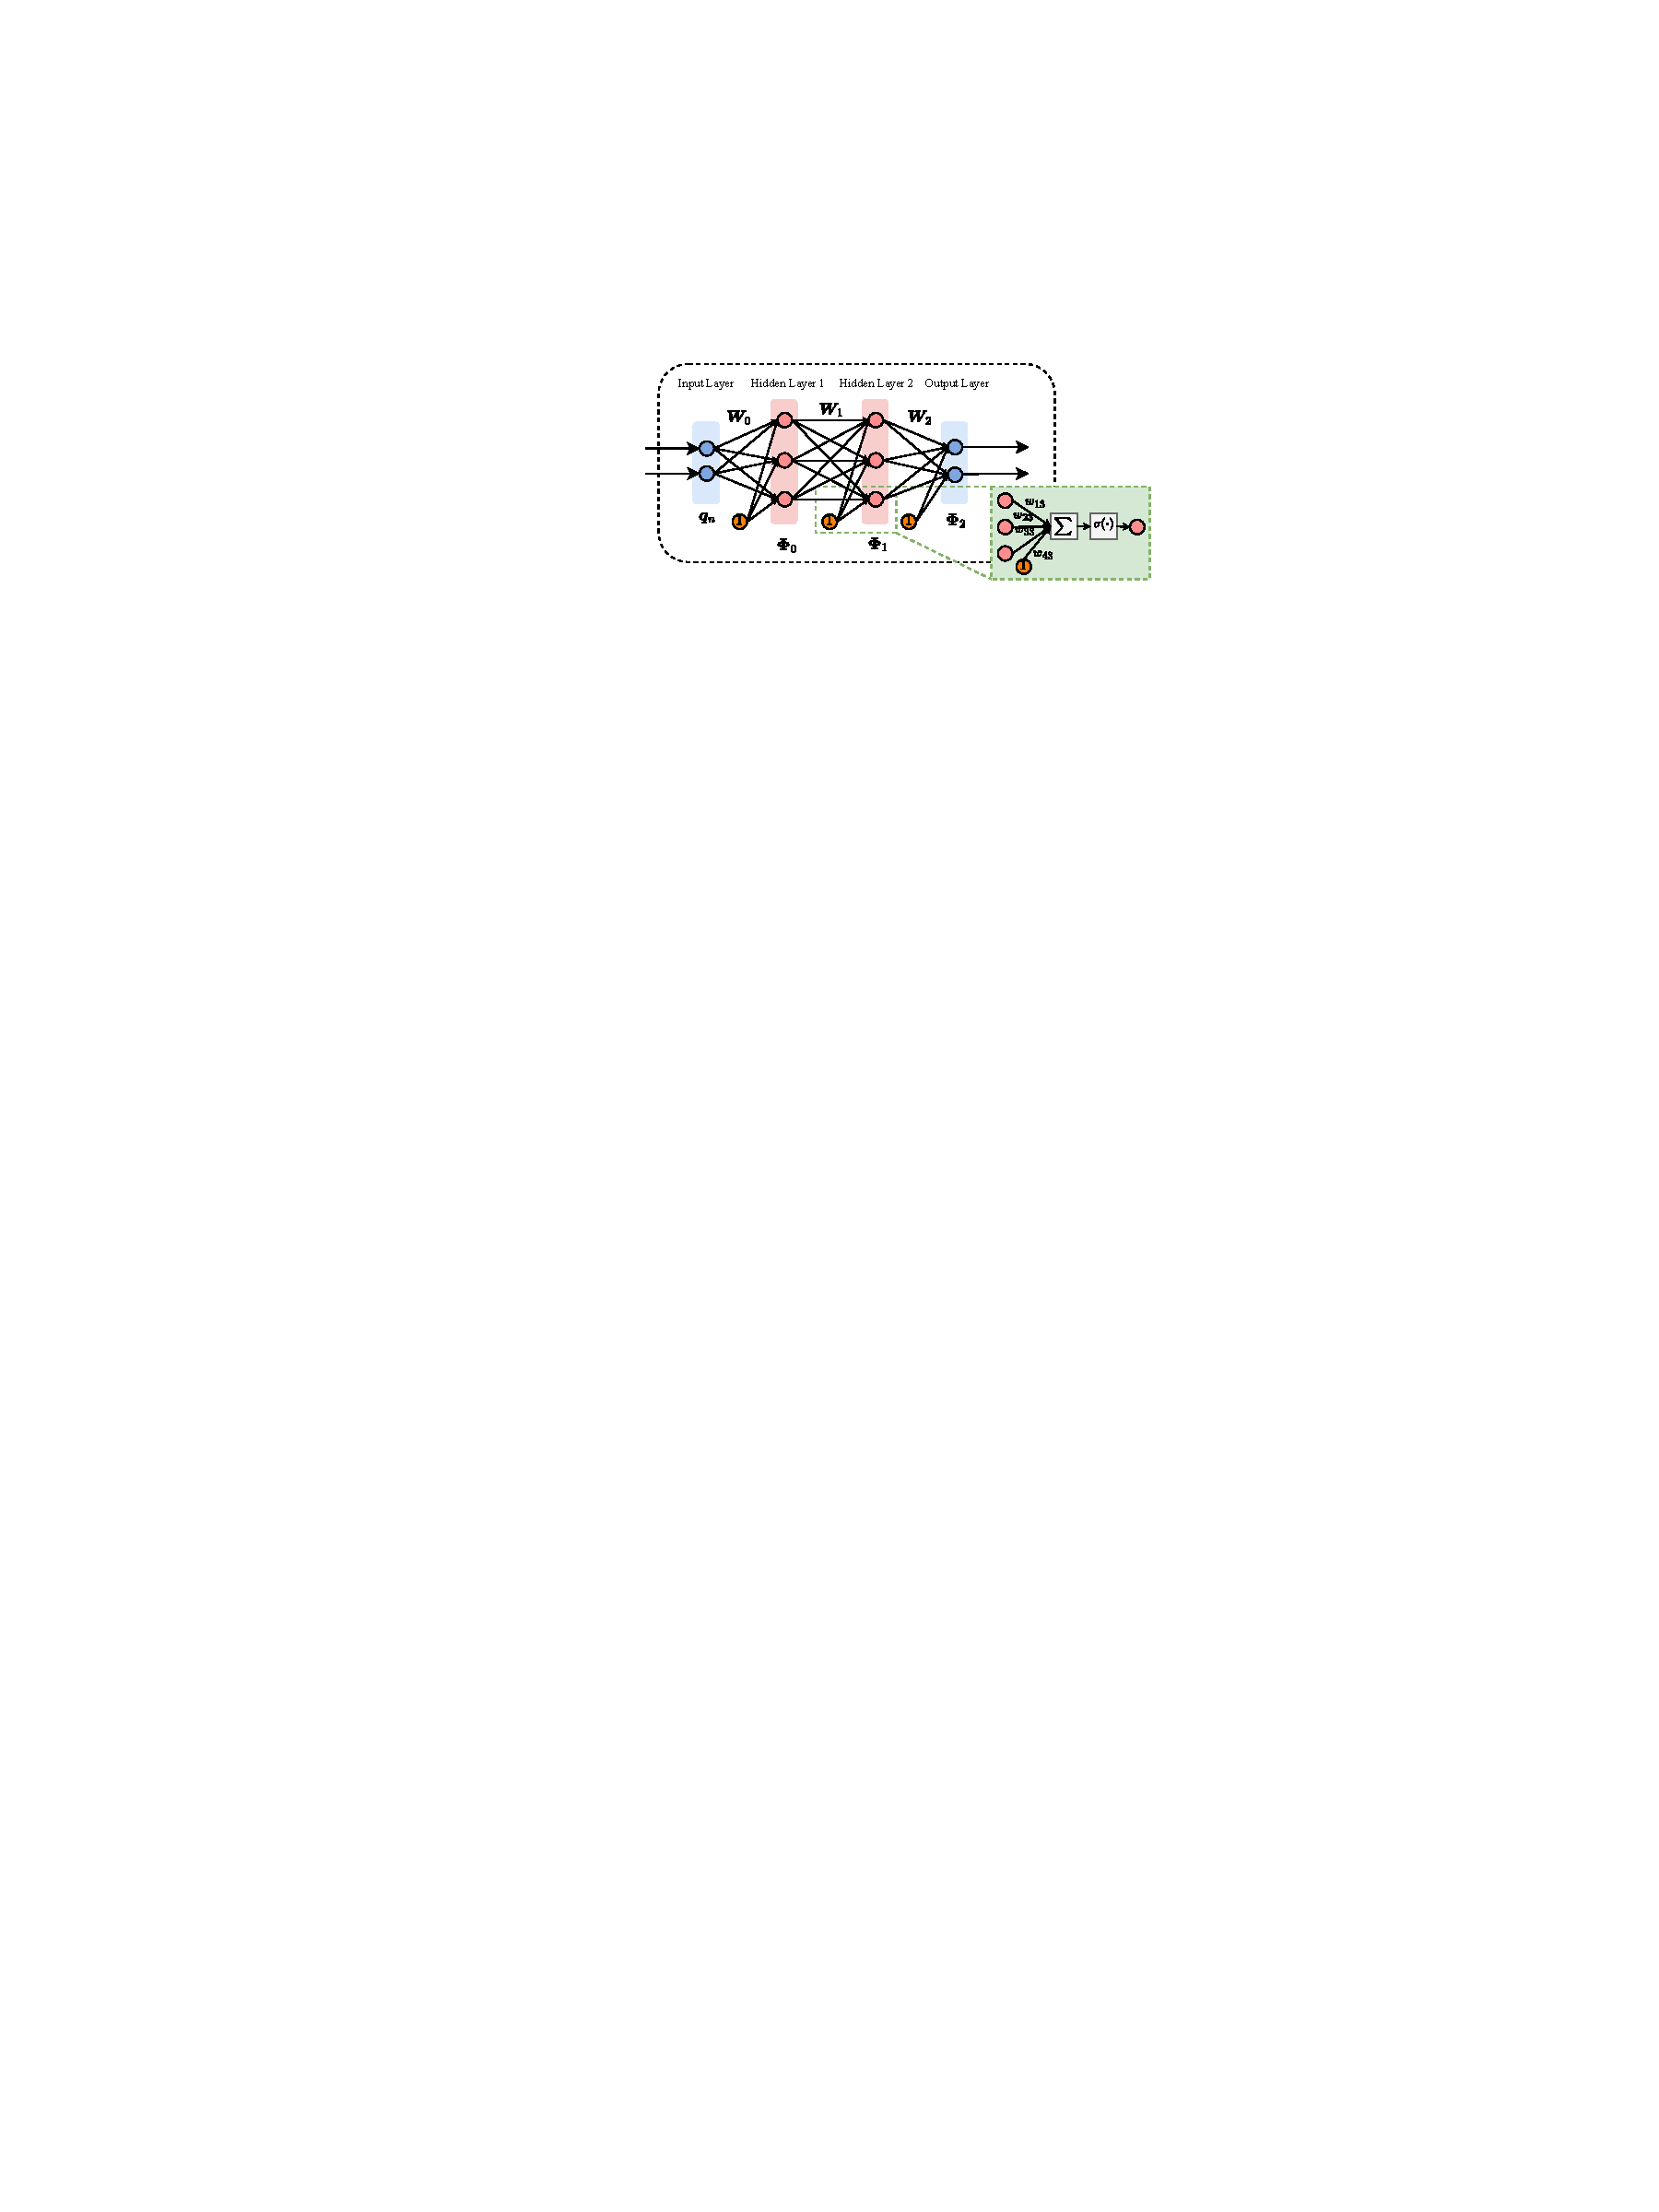
\includegraphics[width=0.7\textwidth]{figures/DNN.drawio.pdf}
        \caption{Architecture of the DNN.}
      \end{figure}
    }

  \end{columns}

    \let\thefootnote\relax\footnote{
      \textit{Notations}: 
        $\mv{q}\in\R^n$: Joint position, $\mm{M}$: Inertia matrix, $\mm{C}$: Coriolis matrix, $\mm{G}$: Gravity vector, $\mv{\tau}$: Control input, $\mv{\tau}_d$: Disturbance.
      }

\end{frame}
%~~~~~~~~~~~~~~~~~~~~~~~~~~~~~~~~~~~~~~~~~~~~~~~~~~~~~~~~~~~~~~~~~~~~~~~~~~~~~~

\note[enumerate]{
  \item The proposed method consists of a DNN and weight optimizer, inside.
  \item Let's start with the system.
  \begin{itemize}
    \item The system is a two-link robotic manipulator system, which is controlled by the control input $\mv{\tau}$.
    \item The control input is saturated by the saturation function $\mysat(\cdot)$.
    \item The desired trajectory $\mv{q}_d$ is given.
  \end{itemize}
  \item The control input is purely decided by the DNN, so the output of the DNN is the control input.
  \item And, the DNN is defined like \eqref{eq:NN}, with $k$ layers and weights, and $\tanh(\cdot)$ as the activation function.
}

% ╔═══════════════════════════════════════════════╗
% ║ Section: Proposed Method                      ║
% ║   - Subsection: Problem Formulation           ║
% ╚═══════════════════════════════════════════════╝
\subsection{Problem Formulation}

%~~~~~~~~~~~~~~~~~~~~~~~~~~~~~~~~~~~~~~~~~~~~~~~~~~~~~~~~~~~~~~~~~~~~~~~~~~~~~~
\begin{frame}{\insertsubsectionhead}{Optimization Problem}

\begin{columns}

  \column{0.45\textwidth}

    \textbf{Optimization Problem Statement}:

    \begin{itemize}
      \item \ctxt{awesome}{Find } NN weights $\estwth$,
      \item That \ctxt{airforceblue}{minimize } objective function $J(\cdot)$,
        \begin{equation}\label{eq:obj}
          J(\mv{r};\estwth)
          := 
          \frac{1}{2} \mv{r}^\top \mv{r}.
        \end{equation}
        \begin{itemize}
          \item where $\mv{r} := \ddt\mv{e} + \Lambda\mv{e}$ is \ctxt{awesome}{filtered tracking error},
        \end{itemize}
      \item while satisfying the following \ctxt{awesome}{constraints}:
        \begin{itemize}
          \item \ctxt{airforceblue}{Boundedness } of the NN weights $\estwth$.
          \item \ctxt{airforceblue}{Saturation } of the control input $\mv{\tau}$.
        \end{itemize}
    \end{itemize}

  
  \column{0.5\textwidth}

  \onslide<2->
  {
    \begin{block}{Considered Constraints}

      \begin{itemize}
        \item \textbf{Weight Boundedness for Each Layer}: 
          \begin{equation}\label{eq:cstr:weight}
            c_{\theta_i}(\estwth)
            :=
            \norm{\estwth_i}^2 - \overline{\theta_i}^2 \le 0
            , 
            \forall i\in\{0,\ldots,k\}
          \end{equation}

        \item \textbf{Convex control Input Saturation}: 
          \begin{itemize}
            \item Input bound constraint \textit{for each control input}:
            \begin{equation}\label{eq:cstr:input_bound}
              c_{\overline{\tau}_i}(\estwth)
              :=
              \tau_i - \overline{\tau_i}
              \le 
              0
              ,
              \quad
              c_{\underline{\tau}_i}(\estwth)
              :=
              \underline{\tau_i} - \tau_i
              \le 
              0
            \end{equation}
            \item Input norm constraint:
            \begin{equation}\label{eq:cstr:input_norm}
              c_{\mv{\tau}}(\estwth)
              :=
              \norm{\mv{\tau}}^2 - \overline{\tau}^2
              \le
              0
            \end{equation}
        \end{itemize}
      \end{itemize}
      
    \end{block}
  }

  \end{columns}

  \let\thefootnote\relax\footnote{
    \textit{Notations}: 
    $\Lambda\in\R_{>0}^{n\times n}$: filtering matrix
  }

\end{frame}
% ~~~~~~~~~~~~~~~~~~~~~~~~~~~~~~~~~~~~~~~~~~~~~~~~~~~~~~~~~~~~~~~~~~~~~~~~~~~~~~
\note[enumerate]
{
  \item The control problem can be represented as a constrained optimization problem.
  \begin{itemize}
    \item That is, 
    \item We need to find NN weights ...
  \end{itemize}
  \item To explicitly consider the constraints, we define the constraint functions as follows, for weight boundedness and convex control input saturation of each control input and norm of the control input.
}

%~~~~~~~~~~~~~~~~~~~~~~~~~~~~~~~~~~~~~~~~~~~~~~~~~~~~~~~~~~~~~~~~~~~~~~~~~~~~~~
\begin{frame}{\insertsubsectionhead}{Optimization Problem}

  \textbf{Original Optimization Problem}

  \begin{itemize}
    \item Constrained optimization problem to minimize the tracking error.
    \item Inequality constraints $c_j(\estwth) \le 0$ for $j\in\mathcal{I}$.
  \end{itemize}

    \begin{equation}\label{eq:opt_problem}
      \begin{matrix}
        \min_{\estwth} J(\mv{r};\estwth)
        \\\ \\
        \text{s.t. } c_{j}(\estwth) 
        \le 
        0
        ,
        \forall j\in\mathcal{I}
      \end{matrix}
    \end{equation}

  \onslide<2->
  {
    \textbf{Define Lagrangian Function}

    \begin{equation}\label{eq:lagrangian}
        L(\mv{r},\estwth,[\lambda_j]_{j\in\mathcal{I}})
        :=
        J(\mv{r};\estwth)
        +
        \sum_{j\in\mathcal{I}} \lambda_j c_j(\estwth)
    \end{equation}
  }

  \onslide<3->
  {
    \textbf{Dual Problem}
    \begin{itemize}
      \item The dual problem is to \ctxt{airforceblue}{minimize } the Lagrangian function with respect to the \ctxt{airforceblue}{NN weights } $\estwth$, while \ctxt{awesome}{maximizing } with respect to the \ctxt{awesome}{Lagrange multipliers } $\lambda_j$.
      \item The Lagrange multipliers $\lambda_j$ are non-negative, \ie $\lambda_j \ge 0$.
    \end{itemize}

    \begin{equation}\label{eq:dual_problem}
      \min_{\estwth}\max_{[\lambda_j]_{j\in\mathcal{I}}} 
      L(\mv{r},\estwth,[\lambda_j]_{j\in\mathcal{I}})
    \end{equation}
  }

\end{frame}
%~~~~~~~~~~~~~~~~~~~~~~~~~~~~~~~~~~~~~~~~~~~~~~~~~~~~~~~~~~~~~~~~~~~~~~~~~~~~~~

\note[enumerate]
{
  \item Then using the constraint functions, we can formulate the constrained optimization problem as in \eqref{eq:opt_problem}.
  \item And, we can define the Lagrangian function as in \eqref{eq:lagrangian}.
  \item So, the dual problem can be formulated as in \eqref{eq:dual_problem}.
  \item It means, that we can find the optimal solution by minimizing the Lagrangian function with respect to the NN weights, while maximizing it with respect to the Lagrange multipliers.
}

% ╔═══════════════════════════════════════════════╗
% ║ Section: Proposed Method                      ║
% ║   - Subsection: Adaptation Law Derivation     ║
% ╚═══════════════════════════════════════════════╝
\subsection{Adaptation Law Derivation}

%~~~~~~~~~~~~~~~~~~~~~~~~~~~~~~~~~~~~~~~~~~~~~~~~~~~~~~~~~~~~~~~~~~~~~~~~~~~~~~
\begin{frame}{\insertsubsectionhead}{Gradient Descent/Ascent Method}
  
  To solve the dual problem, 
  \begin{equation}
    \min_{\estwth}\max_{[\lambda_j]_{j\in\mathcal{I}}} 
    L(\mv{r},\estwth,[\lambda_j]_{j\in\mathcal{I}})
    ,
  \end{equation}
  the first-order gradient descent/ascent method is used to derive the adaptation law.

  \centering
  \begin{minipage}{0.6\textwidth}%

    \begin{block}{Adaptation Law}%
      
    \onslide<2->
    {
      \textbf{Gradient \ctxt{airforceblue}{Descent } Method for weights $\estwth$}:
      \begin{equation}\label{eq:adaptation_law:1}
        \ddtt {
          \ctxt{airforceblue}{\estwth}
          }
        =
        -\alpha 
        \pptfrac{L}{\ctxt{airforceblue}{\estwth}}
        =-\alpha 
        \left(
            \pptfrac{J}{\ctxt{airforceblue}{\estwth}}
            +
            \textstyle\sum_{j\in\mathcal{I}}
            \ctxt{awesome}{\lambda_j}
            \pptfrac{c_j}{\ctxt{airforceblue}{\estwth}}
        \right),
      \end{equation}
    }

    \onslide<3->
    {
      \textbf{Gradient \ctxt{awesome}{Ascent } Method for Lagrange multipliers $\lambda_j, \forall j\in\mathcal I$}:
      \begin{equation}\label{eq:adaptation_law:2}
        \ddtt\ctxt{awesome}{\lambda_j}
        = 
        \beta_j
        \pptfrac{L}{\ctxt{awesome}{\lambda_j}} 
        = 
        \beta_j c_j ,
      \end{equation}
    }

    \onslide<4->
    {
      For non-negativity of the Lagrange multipliers,
      \begin{equation}\label{eq:adaptation_law:3}
        \ctxt{awesome}{\lambda_j}
        \leftarrow
        \max(\ctxt{awesome}{\lambda_j},0)
        .
      \end{equation}
    }

    \end{block}
  \end{minipage}
  
  \let\thefootnote\relax\footnote{
    $\alpha$: adaptation gain (learning rate), $\beta_j$: update rate of the Lagrange multipliers.
  }

\end{frame}
%~~~~~~~~~~~~~~~~~~~~~~~~~~~~~~~~~~~~~~~~~~~~~~~~~~~~~~~~~~~~~~~~~~~~~~~~~~~~~~

\note[enumerate]
{
  \item To solve this problem, we employed the first-order gradient descent/ascent method.
  \item For minimizing the Lagrangian function with respect to the NN weights, the gradient descent method is used.
  \begin{itemize}
    \item We have a adaptation gain $\alpha$ to control the learning rate.
  \end{itemize}
  \item For maximizing the Lagrangian function with respect to the Lagrange multipliers, the gradient ascent method is used.
  \begin{itemize}
    \item We have an update rate $\beta_j$ for each Lagrange multiplier.
  \end{itemize}
  \item Finally, the max operator is used to ensure the non-negativity of the Lagrange multipliers.
  \item Therefore, according to the adaptation law, when the constraints are active, the Lagrange multipliers are updated to be positive.
  \item And, the NN weights are updated to minimize the constraint violation while minimizing the tracking error.
  \item After the constraints are satisfied, \it negative, the Lagrange multipliers are updated to zero, and the NN weights are updated to minimize the tracking error only.
}

% ╔═══════════════════════════════════════════════╗
% ║ Section: Proposed Method                      ║
% ║   - Subsection: Stability Analysis            ║
% ╚═══════════════════════════════════════════════╝
\subsection{Stability Analysis}

%~~~~~~~~~~~~~~~~~~~~~~~~~~~~~~~~~~~~~~~~~~~~~~~~~~~~~~~~~~~~~~~~~~~~~~~~~~~~~~
\begin{frame}{\insertsubsectionhead}{Lyapunov Stability Analysis}

  \centering
  \begin{minipage}{.9\textwidth}

    \begin{block}{Theorem 1 \cite{Ryu:2025aa}}
      For the \ctxt{airforceblue}{dynamical system } described in \eqref{eq:sys}, the \ctxt{awesome}{neuro-adaptive controller } in \eqref{eq:input} with the \ctxt{airforceblue}{weight adaptation laws } in \eqref{eq:adaptation_law:1}, \eqref{eq:adaptation_law:2} and \eqref{eq:adaptation_law:3} ensure the \ctxt{airforceblue}{boundedness } of the \ctxt{awesome}{filtered error } $\mv{r}$ and the \ctxt{awesome}{weight estimate } $\estwth$, under the control input constraints satisfying Assumption 1 and 2. This holds under the \ctxt{awesome}{weight norm constraint } \eqref{eq:cstr:weight}.
    \end{block}

    \begin{exampleblock}{Assumption 1 (Convex Input Constraint)}
      The constraint functions $c_j(\estwth),\forall j\in\mathcal{I}$, are convex in the $\tau$-space and satisfy $c_j(\estwth)\le0$ and $c_j(\idealwth)\le0$.
    \end{exampleblock}

    \begin{exampleblock}{Assumption 2, Linear Independence Constraint Qualification (LICQ)}
      The selected constraints satisfy the Linear Independence Constraint Qualification (LICQ) \cite[Chap. 12 Def. 12.1]{Nocedal:2006aa}.
    \end{exampleblock}

  \end{minipage}

  \vspace{.2cm}

  Proof of Theorem 1 is \textbf{omitted } due to space limitations. The detailed proof can be found in \cite{Ryu:2025aa}.

\end{frame}
%~~~~~~~~~~~~~~~~~~~~~~~~~~~~~~~~~~~~~~~~~~~~~~~~~~~~~~~~~~~~~~~~~~~~~~~~~~~~~~

\note[enumerate]
{
  \item The stability of the proposed methods is proven using Lyapunov stability theory.
  \item The requirements for the stability are as follows.
  \item First, the weight norm constraints should be imposed.
  \item And, two assumptions for convex input constraints and LICQ conditions should be satisfied.
  \item The proof is omitted, but the detailed proof can be found in the reference \cite{Ryu:2025aa}.
}

% ╔═══════════════════════════════════════════════╗
% ║ Section: Experimental Validation              ║
% ╚═══════════════════════════════════════════════╝

\section{Experimental Validation}

% ╔═══════════════════════════════════════════════╗
% ║ Section: Experimental Validation              ║
% ║   - Subsection: Simulation Setup              ║
% ╚═══════════════════════════════════════════════╝
\subsection{Simulation Setup}

%~~~~~~~~~~~~~~~~~~~~~~~~~~~~~~~~~~~~~~~~~~~~~~~~~~~~~~~~~~~~~~~~~~~~~~~~~~~~~~
\begin{frame}{\insertsubsectionhead}{Two-Link Robotic Manipulator}

    \begin{columns}

      \column{.45\textwidth}

        \textbf{Target System}:

        \begin{equation*}
          \mm{M}\ddq + \mm{V}_m\dq + \mv{F} + \mv{G} + \mv{\tau}_d
          =
          \mv{\tau}
        \end{equation*}

        \begin{figure}
          \centering
          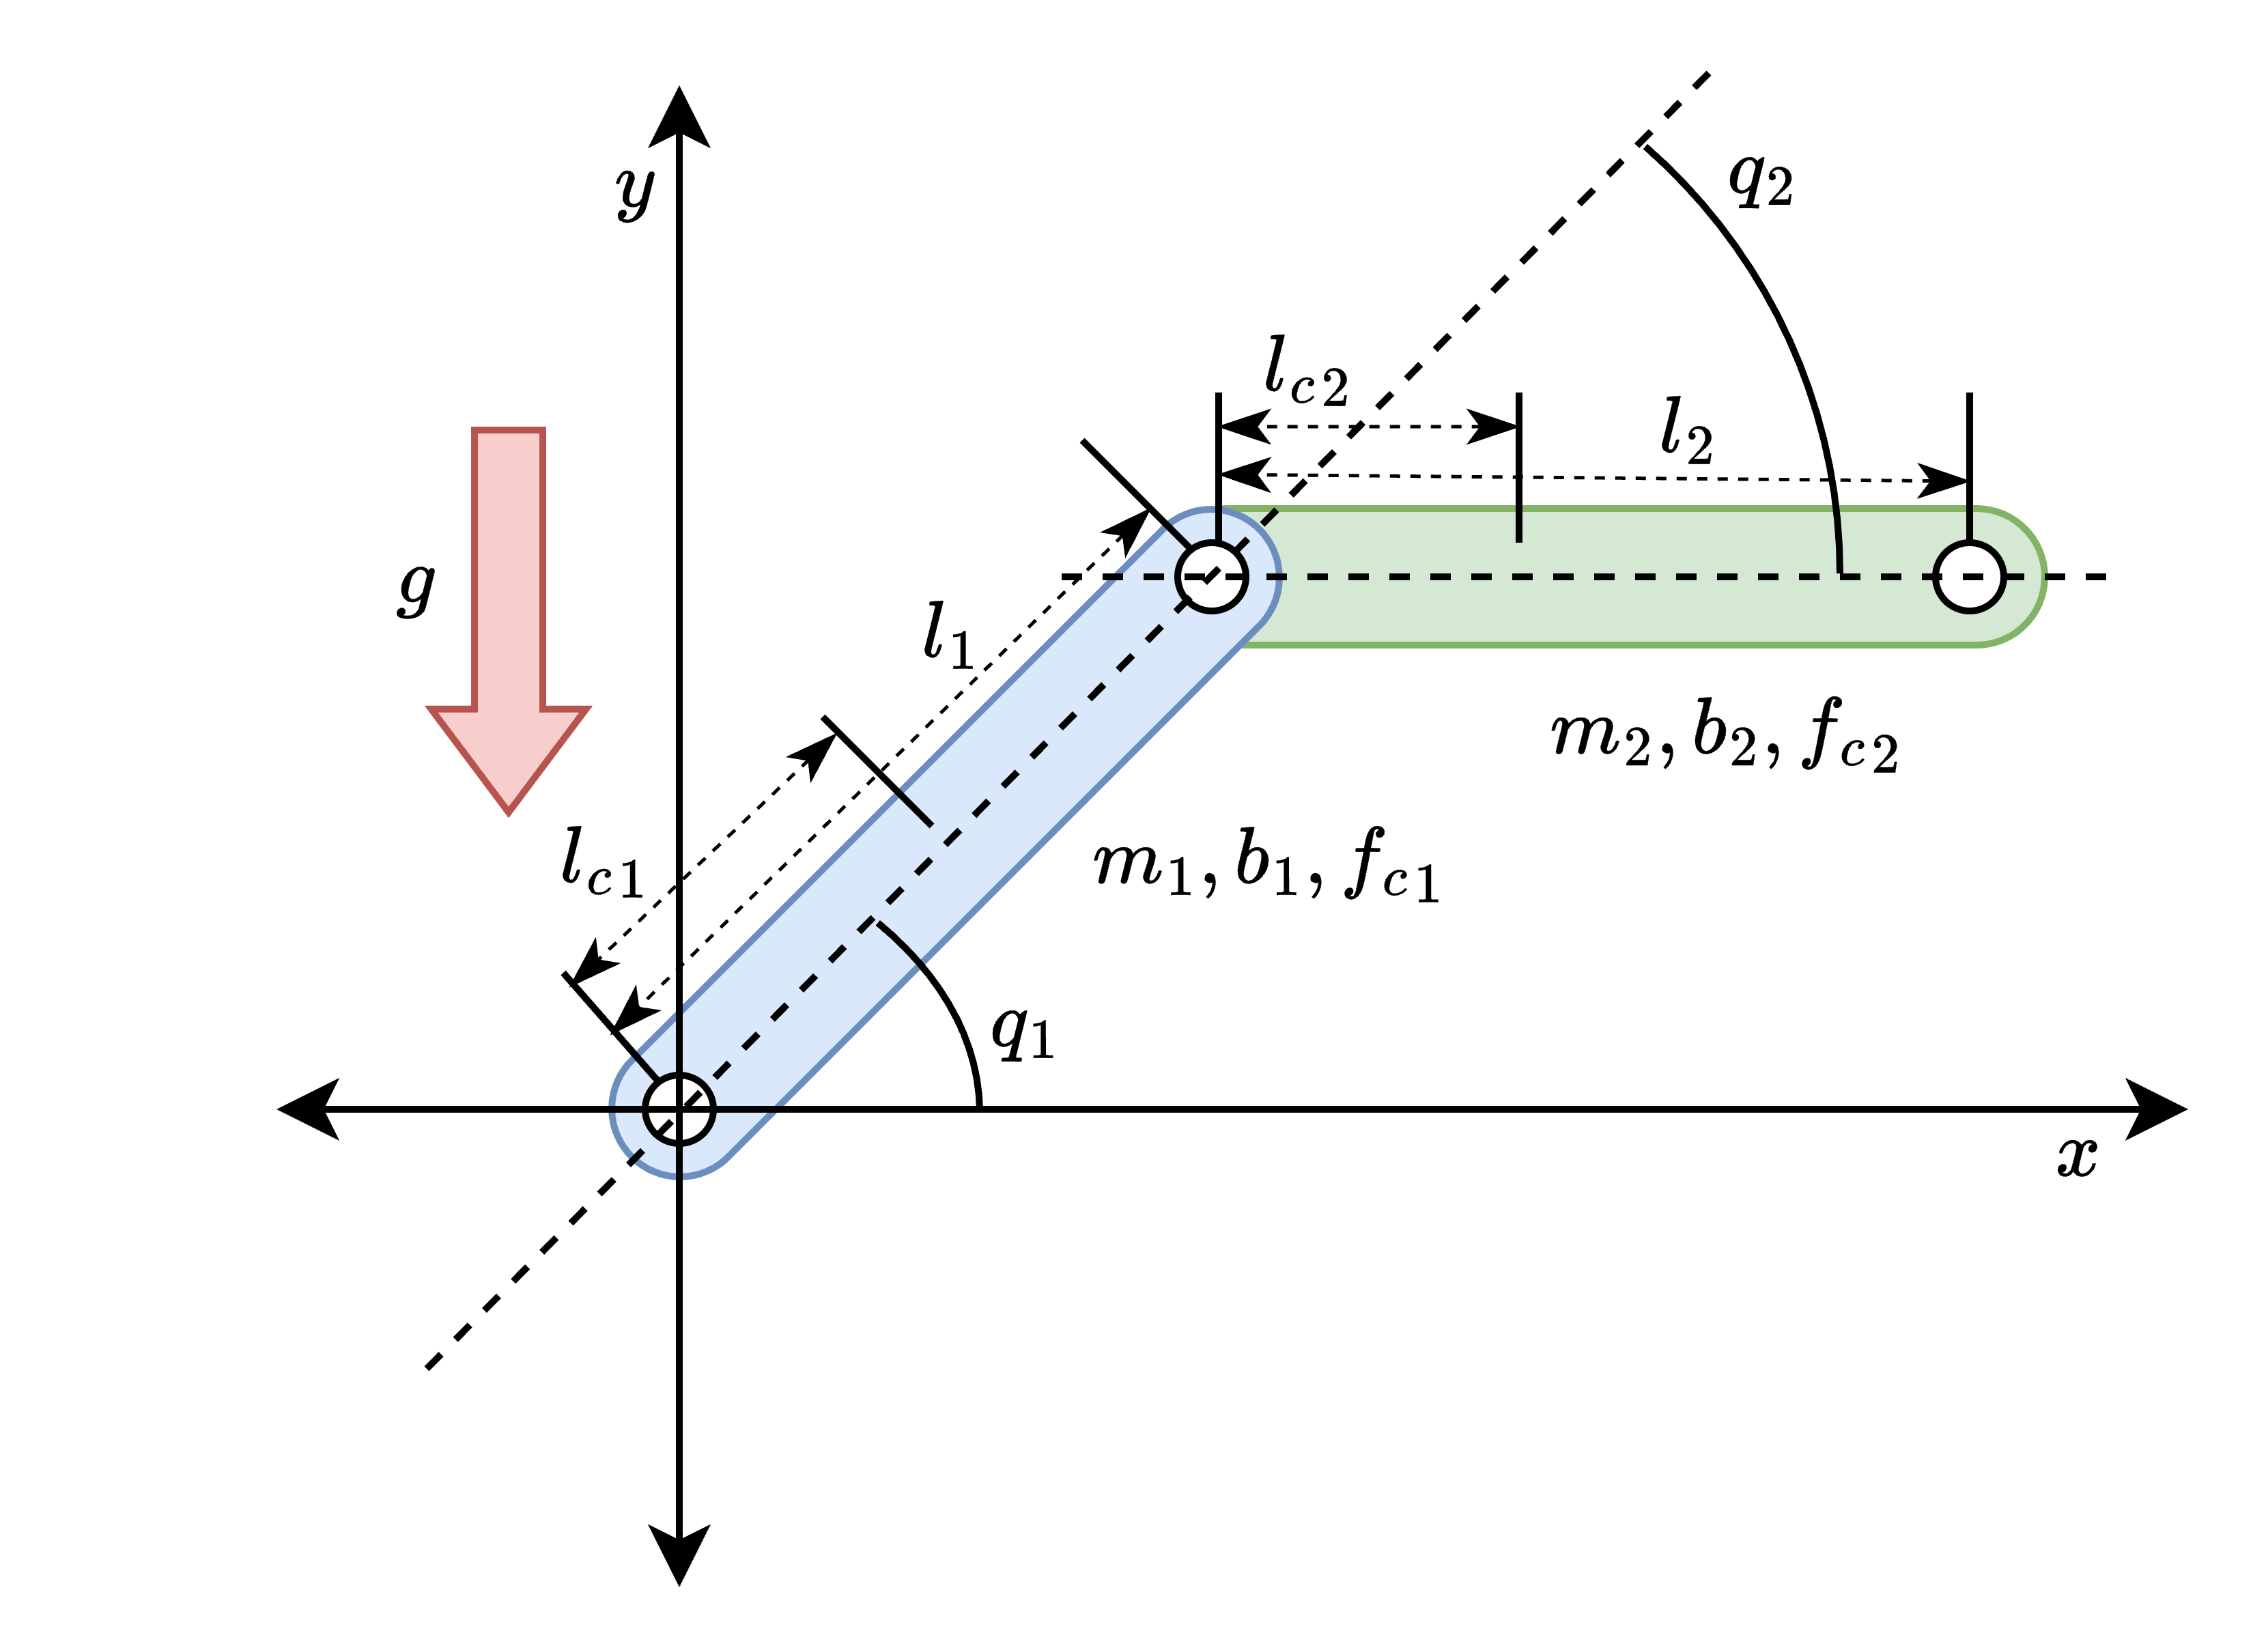
\includegraphics[width=.99\textwidth]{figures/RobotModel.drawio.png}
          \caption{Two-link robotic manipulator model.}
        \end{figure}

      \column{.55\textwidth}
      
        \textbf{Desired Trajectory}:

        \begin{equation}
          \qd
          =
          \begin{pmatrix}
              {q_d}_1\\
              {q_d}_2
          \end{pmatrix}
          = 
          \begin{pmatrix}
              +\cos(
                  \tfrac{\pi}{2}t
              ) + 1 \\
              -\cos(
                  \tfrac{\pi}{2}t
              ) - 1 
          \end{pmatrix}
          .
      \end{equation}

      \textbf{System Model Parameters}:

      \begin{table}
        \renewcommand{\arraystretch}{1.3}
        \caption{System model parameters.}
        \centering
        \begin{tabular}{c m{5em} c c c }
        \hline
        \textbf{Symbol} & \textbf{Description} & \textbf{Link 1} & \textbf{Link 2} \\
        \hline
        \hline 
        $m_p$ & Mass & 23.902 kg & 3.88 kg \\
        \hline
        $l_p$  & Length & 0.45 m & 0.45 m \\
        \hline
        ${l_c}_p$ & COM & 0.091 m & 0.048 m \\
        \hline
        $b_p$   & Viscous coef. &  2.288 Nms & 0.172 Nms \\
        \hline
        ${f_c}_p$  & Friction coef. & 7.17 Nm & 1.734 Nm \\
        \hline
        \end{tabular}
        \label{table: system parameters}
      \end{table}

    \end{columns}

\end{frame}
%~~~~~~~~~~~~~~~~~~~~~~~~~~~~~~~~~~~~~~~~~~~~~~~~~~~~~~~~~~~~~~~~~~~~~~~~~~~~~~

\note[enumerate]
{
  \item For validation, we simulated a two-link robotic manipulator system.
  \item A simple cosine trajectory is given as the desired trajectory.
}

%~~~~~~~~~~~~~~~~~~~~~~~~~~~~~~~~~~~~~~~~~~~~~~~~~~~~~~~~~~~~~~~~~~~~~~~~~~~~~~
\begin{frame}{\insertsubsectionhead}{Controllers Setting}
  
  \begin{itemize}
    \item Only \ctxt{awesome}{weight norm constraint } is considered in this presentation (for \textbf{ECC}).
    \item Input saturation constraints are not considered.
    \item For simplicity, \ctxt{airforceblue}{single hidden layer NN} is used.
  \end{itemize}

  \centering
  \begin{figure}
    \includegraphics[width=0.8\textwidth]{figures/Controller.drawio.pdf}
    \caption{Architecture of the controllers.}
  \end{figure}

\end{frame}
%~~~~~~~~~~~~~~~~~~~~~~~~~~~~~~~~~~~~~~~~~~~~~~~~~~~~~~~~~~~~~~~~~~~~~~~~~~~~~~

\note[enumerate]
{
  \item For this conference paper, we only considered the weight norm constraint.
  \item So, please ignore the input saturation.
}

%~~~~~~~~~~~~~~~~~~~~~~~~~~~~~~~~~~~~~~~~~~~~~~~~~~~~~~~~~~~~~~~~~~~~~~~~~~~~~~
\begin{frame}{\insertsubsectionhead}{Controllers for Comparative Study}
  
    \begin{itemize}
      \item NAC-CO denotes the proposed controller based on \ctxt{airforceblue}{constrained optimization }.
      \item For NAC-L2 and NAC-eMod, the \ctxt{awesome}{stabilizing terms } $-\lambda\estwth$ and $\rho\norm{\mv{r}}\estwth$ ensures the weights boundedness, respectively.
    \end{itemize}

    \begin{table}
      \renewcommand{\arraystretch}{1.5}
      % \caption{Controller Properties.}
      \centering
      \begin{tabular}{c m{20em} c c c }
      \hline
      \textbf{Name} & \textbf{Description} & \textbf{Adaptation Law} \\
      \hline
      \hline 
        \multirow{2}{*}{NAC-L2} & NAC with $L_2$-regularization \tiny{(equal to $\sigma$-modification)} & \multirow{2}{*}
        {$
          \ddt\estwth = -\alpha \left(\ppfrac{J}{\estwth}+\ctxt{awesome}{\lambda}\estwth\right)
        $}
        \\
          & ($\ctxt{awesome}{\lambda}$ stabilizes $\estwth$ towards origin) &
        \\
      \hline
        \multirow{2}{*}{NAC-eMod} & NAC with $\epsilon$-modification & \multirow{2}{*}
        {$
          \ddt\estwth = -\alpha \left(\ppfrac{J}{\estwth}+\ctxt{awesome}{\rho}\norm{\tilde{\mv{r}}}\estwth\right)
        $}
        \\
        & ($\ctxt{awesome}{\rho}$ stabilizes proportionally to filtered error $\mv{r}$) &
        \\
      \hline
        \multirow{2}{*}{NAC-CO} & Constrained Optimization-based NAC & 
        $
          \ddt\estwth = -\alpha \left(\ppfrac{J}{\estwth}+\sum_{j\in\mathcal{I}}\lambda_j\ppfrac{c_j}{\estwth}\right)
        $ 
        \\
          (proposed) & ($\ctxt{awesome}{\beta_j}$ determines $\lambda_j$ adaptation speed) &
        $
          \ddt\lambda_j = \ctxt{awesome}{\beta_j} c_j$, and $\lambda_j \leftarrow \max(\lambda_j,0)
        $
        \\
      \hline
      \end{tabular}
      \label{table:sys:param}
    \end{table}

    \onslide<2->
    {
      \centering
      \begin{minipage}{0.75\textwidth}
        \begin{block}{Simulation Objective}
          By \ctxt{airforceblue}{varying the parameters }, \ie $\beta_j$, $\lambda$, and $\rho$, the parameter dependencies will be investigated.
        \end{block}
      \end{minipage}
    }

\end{frame}
%~~~~~~~~~~~~~~~~~~~~~~~~~~~~~~~~~~~~~~~~~~~~~~~~~~~~~~~~~~~~~~~~~~~~~~~~~~~~~~

\note[enumerate]
{
  \item For comparative study, we used two existing methods: L2-regularization (NAC-L2) and $\epsilon$-modification (NAC-eMod).
  \item Please, note that the L2-regularization is equal to the $\sigma$-modification.
  \item In summary, the NAC-L2 and NAC-eMod use the stabilizing terms $-\lambda\estwth$ and $\rho\norm{\mv{r}}\estwth$, respectively, to ensure the boundedness of the weights.
  \item While the NAC-CO is the proposed method, which uses the Lagrange multipliers $\lambda_j$ to ensure the boundedness of the weights.
  \item The simulation is mainly conducted to investigate dependencies of the crucial parameters, \ie $\beta_j$, $\lambda$, and $\rho$.
}

% ╔═══════════════════════════════════════════════╗
% ║ Section: Experimental Validation              ║
% ║   - Subsection: Simulation Results            ║
% ╚═══════════════════════════════════════════════╝
\subsection{Simulation Results}

%~~~~~~~~~~~~~~~~~~~~~~~~~~~~~~~~~~~~~~~~~~~~~~~~~~~~~~~~~~~~~~~~~~~~~~~~~~~~~~
\begin{frame}{\insertsubsectionhead}{Box-and-Whisker Plots}
  
  \begin{columns}
    \column{0.6\textwidth}
    
      \textbf{Parameter Dependencies Investigation}:
      
      \small
      {
        \begin{itemize}
          \item<+-> The parameters ranged from $0.001$ to $1$ across 10 samples.
          \item<+-> NAC-L2 shows the \ctxt{awesome}{worst performance } with high variance.
          \item<+-> NAC-CO (proposed) shows the \ctxt{airforceblue}{best performance } and \ctxt{airforceblue}{lowest variance}.
          \item<+-> This result is because, 
            \begin{itemize}
              \item<+-> NAC-L2 and NAC-eMod are \ctxt{airforceblue}{biased towards the origin}. $\ddtt\estwth=-\alpha(\pptfrac{J}{\estwth}+\ctxt{awesome}{\lambda\estwth})$ (NAC-L2) or $+\ctxt{awesome}{\rho\norm{\mv{r}}\estwth}$ (NAC-eMod), proportionally to $\lambda$ and $\rho$, respectively.
              % \item<+-> $\beta_j$ in NAC-CO (proposed) only determines the \ctxt{airforceblue}{update speed } of the Lagrange multipliers $\lambda_j$, \ie $\ddtt\lambda_j=\beta_j c_j$.
              % \begin{itemize}
                \item<+-> $\ctxt{awesome}{-\lambda_j\pptfrac{c_j}{\estwth}}$ in NAC-CO (proposed) (\ie $\ddtt\estwth=-\alpha(\pptfrac{J}{\estwth}+\ctxt{awesome}{\lambda_j\pptfrac{c_j}{\estwth}})$) \ctxt{airforceblue}{disappears } when constraints are inactive (\ie $c_j<0$, and $\lambda=\beta_jc_j$ and $\lambda_j\leftarrow\max(\lambda_j,0)$). %
              % \end{itemize}
            \end{itemize}
        \end{itemize}
      }

    \column{0.4\textwidth}

      \begin{figure}
        \includegraphics[width=.89\textwidth]{figures/BoxWhisker.drawio.png}
        \caption{Box-and-whisker plots of the tracking error ISE.}
      \end{figure}

  \end{columns}

    \begin{table}[!t]
      \renewcommand{\arraystretch}{1.1}
      % \caption{Quantitative comparison of square root of tracking ISE.}
      \centering
      \begin{tabular}{c c c c }
      \hline
      & \textbf{NAC-L2}\!&\!\textbf{NAC-eMod}\!&\!\textbf{NAC-CO} (proposed) 
      \\
      \hline
      \hline 
        Maximum & \ctxt{awesome}{$11.1753 \times\!10^{-3}$} & $0.5603 \times 10^{-3}$ & \ctxt{airforceblue}{$0.3439 \times 10^{-3}$}  \\
      \hline
        Median & \ctxt{awesome}{$0.5898\times\!10^{-3}$}  & $0.5519 \times 10^{-3}$ & \ctxt{airforceblue}{$0.3240 \times 10^{-3}$}  \\
      \hline
        Minimum & \ctxt{awesome}{$0.5434\times\!10^{-3}$}  & $0.5434 \times 10^{-3}$ & \ctxt{airforceblue}{$0.3235 \times 10^{-3}$}  \\
      \hline
      \end{tabular}
      \label{table: error norm}
    \end{table}
    
    \let\thefootnote\relax\footnote{
      Squared root of the tracking error ISE (Integral of Squared Error), \ie $\sqrt{\int_0^T \norm{\mv{r}}^2\,\der t}$, where $T$ denotes a simulation time.
    }
    
\end{frame}
%~~~~~~~~~~~~~~~~~~~~~~~~~~~~~~~~~~~~~~~~~~~~~~~~~~~~~~~~~~~~~~~~~~~~~~~~~~~~~~

\note[enumerate]
{
  \item The parameters were varied from $0.001$ to $1$ across 10 samples.
  \item The box-and-whisker plots show the distribution of the tracking error ISE (Integral of Squared Error).
  \item The NAC-L2 shows the worst performance with high variance, while the NAC-CO (proposed) shows the best performance with the lowest variance.
  \item The reason is that the NAC-L2 and NAC-eMod are biased towards the origin, especially, proportionally to the parameters $\lambda$ and $\rho$, respectively.
  \item On the other hand, the term that biases the weights towards the origin in NAC-CO, is removed when the constraints are inactive, \ie $c_j<0$.
  \item Therefore, the NAC-CO can track the desired trajectory without being biased, when the constraints are inactive.
}

%~~~~~~~~~~~~~~~~~~~~~~~~~~~~~~~~~~~~~~~~~~~~~~~~~~~~~~~~~~~~~~~~~~~~~~~~~~~~~~
\begin{frame}{\insertsubsectionhead}{Weight Norms}

  \begin{columns}

    \column{0.33\textwidth}

      \begin{figure}      
        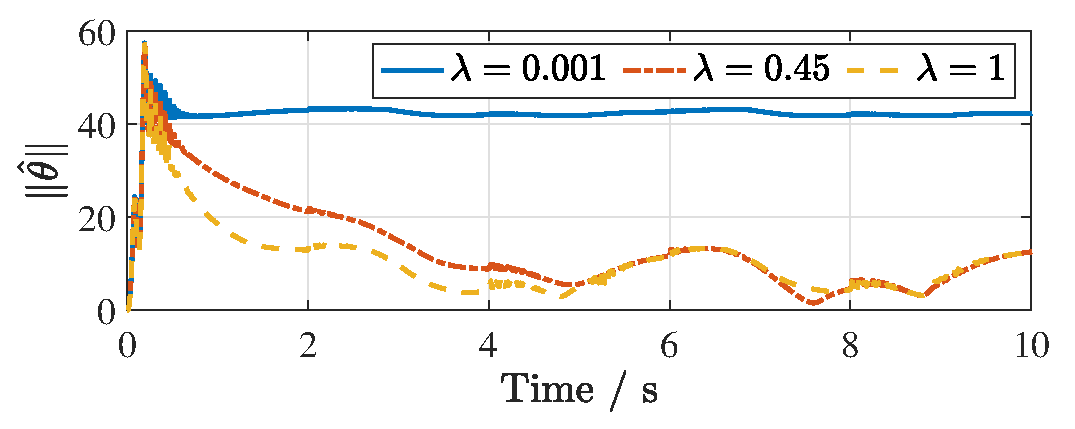
\includegraphics[width=0.99\textwidth]{figures/ECC/fig9.eps}
        \caption{Weight norms of NAC-L2}
      \end{figure}
      
    \column{0.33\textwidth}

      \begin{figure}
        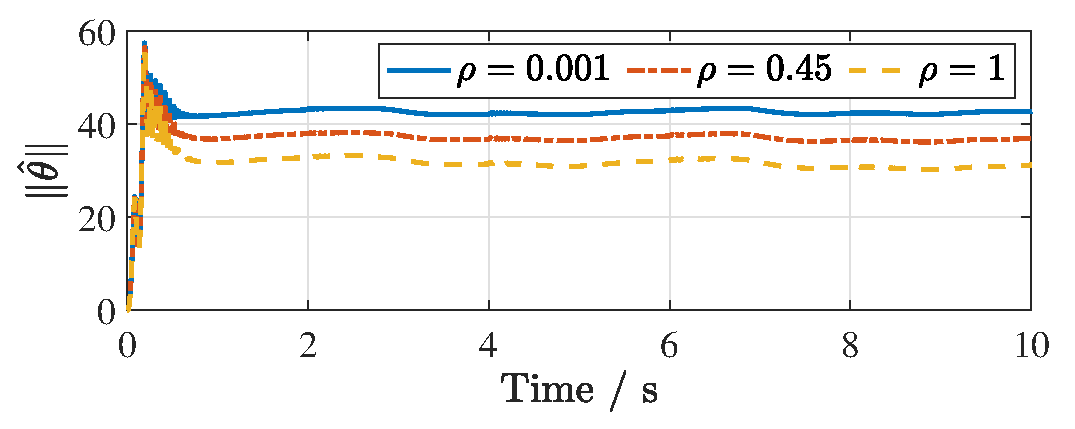
\includegraphics[width=0.99\textwidth]{figures/ECC/fig10.eps}
        \caption{Weight norms of NAC-eMod}
      \end{figure}

    \column{0.33\textwidth}

      \begin{figure}
        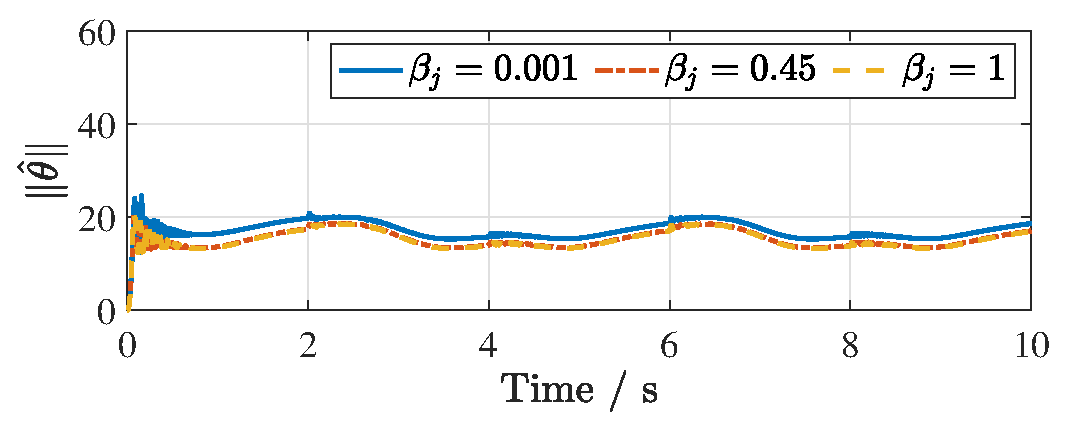
\includegraphics[width=0.99\textwidth]{figures/ECC/fig8.eps}
        \caption{Weight norms of NAC-CO (proposed)}
      \end{figure}
      
  \end{columns}

  \begin{itemize}
    \item<+-> NAC-CO (proposed) showed the \ctxt{airforceblue}{weight norms } are bounded \ctxt{awesome}{under pre-defined constraint } $\overline{\theta}=20$.
    \item<+-> NAC-L2 and NAC-eMod showed the bounded weight norms, but they \ctxt{awesome}{depended } on the parameters $\lambda$ and $\rho$, respectively.
    % \item<+-> As the parameters $\lambda$ and $\rho$ increase, the weight norms of NAC-L2 and NAC-eMod biased towards the origin, which may lead to suboptimal performance.
    \item<+-> In other words, NAC-CO tracked the desired trajectory with a \ctxt{airforceblue}{smaller weight } norm than NAC-L2 and NAC-eMod.
  \end{itemize}

\end{frame}
%~~~~~~~~~~~~~~~~~~~~~~~~~~~~~~~~~~~~~~~~~~~~~~~~~~~~~~~~~~~~~~~~~~~~~~~~~~~~~~

\note[enumerate]
{
  \item In this slide, the weight norms are shown.
  \item We can see that the NAC-CO's weights are bounded under the pre-defined constraint $\overline{\theta}=20$.
  \item The other two methods shows larger weight norms, and biased weights towards the origin, which may lead to suboptimal performance.
  \item Moreover, the dependencies also can be seen, as the distribution of the weight norms of NAC-L2 and NAC-eMod are wider than that of NAC-CO.
}

%~~~~~~~~~~~~~~~~~~~~~~~~~~~~~~~~~~~~~~~~~~~~~~~~~~~~~~~~~~~~~~~~~~~~~~~~~~~~~~
\begin{frame}{\insertsubsectionhead}{Tracking Performance}

  \begin{columns}
    
    \column{0.33\textwidth}

      \begin{figure}      
        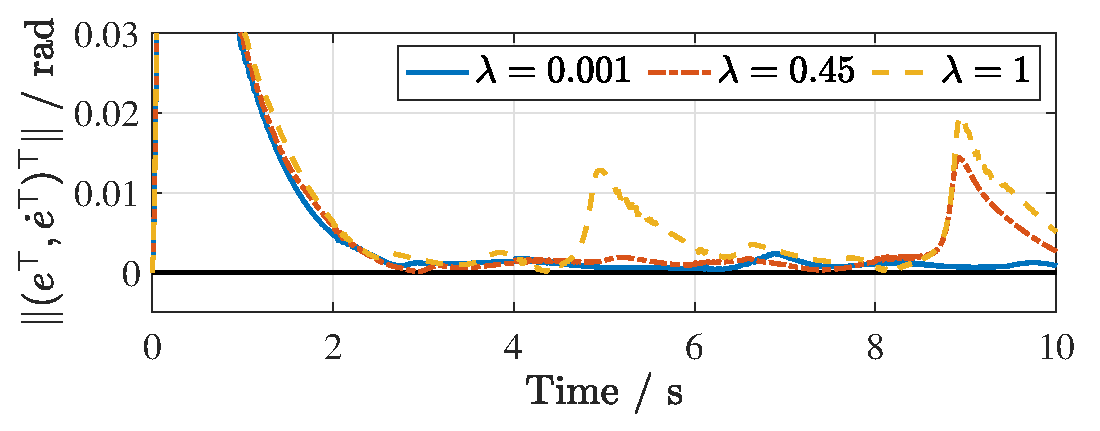
\includegraphics[width=0.99\textwidth]{figures/ECC/fig6.eps}
        \caption{Tracking error of NAC-L2}
      \end{figure}
      
    \column{0.33\textwidth}

      \begin{figure}
        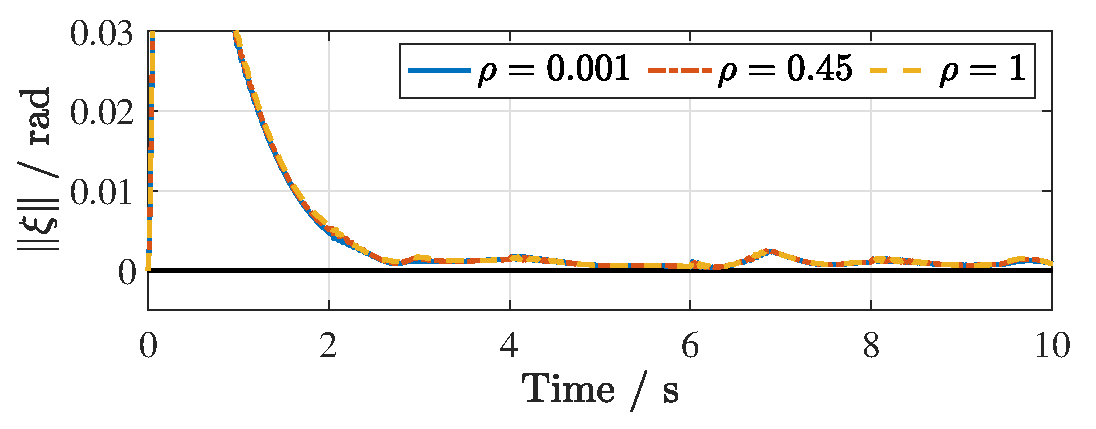
\includegraphics[width=0.99\textwidth]{figures/ECC/fig7.eps}
        \caption{Tracking error of NAC-eMod}
      \end{figure}

    \column{0.33\textwidth}

      \begin{figure}
        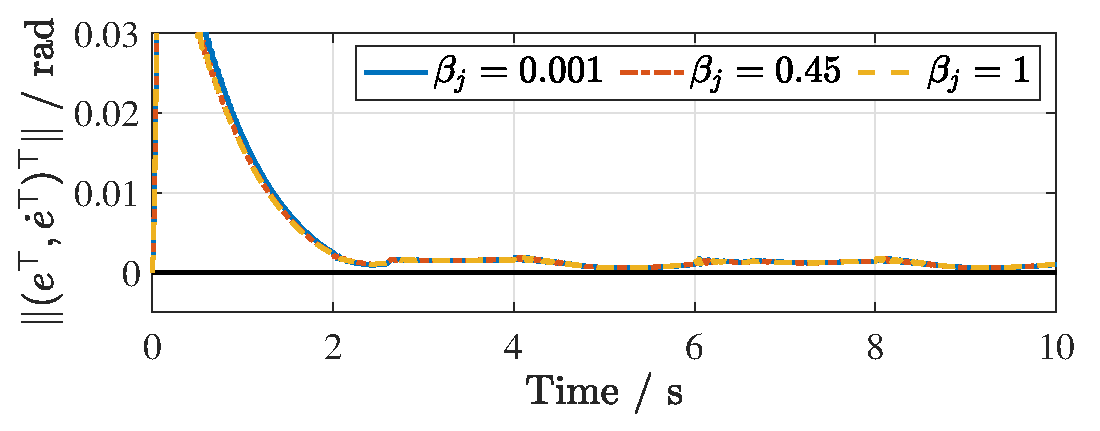
\includegraphics[width=0.99\textwidth]{figures/ECC/fig5.eps}
        \caption{Tracking error of NAC-CO (proposed)}
      \end{figure}

  \end{columns}

  \begin{itemize}
    \item NAC-CO (proposed) \ctxt{airforceblue}{outperformed } NAC-L2 and NAC-eMod in terms of \ctxt{awesome}{tracking performance}.
    \item As the weights are \ctxt{awesome}{biased }towards the origin proportionally to the parameters $\lambda$ and $\rho$ in NAC-L2 and NAC-eMod, respectively, the tracking performance of NAC-L2 and NAC-eMod deteriorated, as approaching toward \ctxt{airforceblue}{suboptimal points}.
  \end{itemize}

\end{frame}
%~~~~~~~~~~~~~~~~~~~~~~~~~~~~~~~~~~~~~~~~~~~~~~~~~~~~~~~~~~~~~~~~~~~~~~~~~~~~~~

\note[enumerate]
{
  \item The tracking performance of the three methods are shown.
  \item The NAC-CO (proposed) outperformed the other two methods in terms of tracking performance.
  \item As the weights are biased towards the origin proportionally to the parameters $\lambda$ and $\rho$ in NAC-L2 and NAC-eMod, respectively, the tracking performance of NAC-L2 and NAC-eMod deteriorated, as approaching toward suboptimal points.
}

%~~~~~~~~~~~~~~~~~~~~~~~~~~~~~~~~~~~~~~~~~~~~~~~~~~~~~~~~~~~~~~~~~~~~~~~~~~~~~~
\begin{frame}{Real-time Implementation Result}

  \begin{itemize}
    \item This video demonstrates:
    \begin{itemize}
      \item \ctxt{airforceblue}{Applicability }of the proposed method to real-time control (under 4 ms sampling time).
      \item \ctxt{awesome}{Convex input constraints } handling.
    \end{itemize}
  \end{itemize}

  \centering
  \includemedia[
      width=0.64\linewidth,
      height=0.36\linewidth,
      activate=onclick,
      addresource=animation.mp4,
      flashvars={
        source=animation.mp4
        &autoPlay=true
        &loop=true
      }
    ]{}{VPlayer.swf}

\end{frame}
%~~~~~~~~~~~~~~~~~~~~~~~~~~~~~~~~~~~~~~~~~~~~~~~~~~~~~~~~~~~~~~~~~~~~~~~~~~~~~~

\note[enumerate]
{
  \item And, until the last slice, we have shown the conference paper's results.
  \item In this slide, we show the recent result with real-time implementation.
  \item The video demonstrates the applicability of the proposed method to real-time control, under 4 ms sampling time.
  \item And, the convex input constraints are handled, here.
}

% ╔═══════════════════════════════════════════════╗ 
% ║ Section: Conclusion and Future Work           ║
% ╚═══════════════════════════════════════════════╝

\section{Conclusion}

\subsection{Conclusion and Future Work}

%~~~~~~~~~~~~~~~~~~~~~~~~~~~~~~~~~~~~~~~~~~~~~~~~~~~~~~~~~~~~~~~~~~~~~~~~~~~~~~
\begin{frame}{Conclusion}
    
  \textbf{Summary of Contributions}
  \begin{itemize}
    \item Proposed a novel constrained optimization-based neuro-adaptive control (CONAC) method.
    \item Adaptation laws are derived using \ctxt{airforceblue}{constrained optimization method}.
    \item The proposed method guarantees the \ctxt{awesome}{stability }of the system and the boundedness of the NN weights.
    \item Feasibility of the proposed method is validated through numerical simulations.
  \end{itemize}

  \textbf{Future Work}
  \begin{itemize}
    \item Extend the proposed method to \ctxt{airforceblue}{state constraints}.
    \item Enhance the \ctxt{awesome}{robustness }and \ctxt{awesome}{flexibility }of the proposed method for \ctxt{airforceblue}{various systems}.
  \end{itemize}

\end{frame}
%~~~~~~~~~~~~~~~~~~~~~~~~~~~~~~~~~~~~~~~~~~~~~~~~~~~~~~~~~~~~~~~~~~~~~~~~~~~~~~

%~~~~~~~~~~~~~~~~~~~~~~~~~~~~~~~~~~~~~~~~~~~~~~~~~~~~~~~~~~~~~~~~~~~~~~~~~~~~~~

\section{}
\begin{frame}{}
    \centering \Large
    \emph{Thank you for your attention!}
\end{frame}
%~~~~~~~~~~~~~~~~~~~~~~~~~~~~~~~~~~~~~~~~~~~~~~~~~~~~~~~~~~~~~~~~~~~~~~~~~~~~~~

%~~~~~~~~~~~~~~~~~~~~~~~~~~~~~~~~~~~~~~~~~~~~~~~~~~~~~~~~~~~~~~~~~~~~~~~~~~~~~~
\begin{frame}[allowframebreaks]{References}

  \bibliography{localRefs}
  \bibliographystyle{IEEEtran}

\end{frame}
%~~~~~~~~~~~~~~~~~~~~~~~~~~~~~~~~~~~~~~~~~~~~~~~~~~~~~~~~~~~~~~~~~~~~~~~~~~~~~~

\end{document}